\documentclass{report}

\usepackage{graphicx}
\usepackage{amsmath}

\title{\textbf{Statistics - Week 4 Questions}\\Owen Burke, 15316452}
\begin{document}
	\maketitle
	\section*{\hfil Question 1 \hfil}
    Consider an experiment where we roll two 6-sided dice. Let random variable Y be the sum of the values rolled. The sample space is \{(1,1),(1,2),(1,3), . . .,(6,6)\} and recall that a 
    random event is a subset of the sample space.
		\subsection*{a)What random event corresponds to Y = 2 ?}
		
        Random variables define a quantity that is associated with a random event but which is real-valued. A random variable is a function that maps from the sample space S 
        to the real line R.\\
        From the question the random variable Y is defined as the sum of the values rolled from the two 6-sided dice.\\
        So, for example, when Y = 6, this denotes the event that the numbers from the two dice add up to the number 6.\\
        Likewise, and for the purpose of this question, when Y = 2, this corresponds to the event that the numbers rolled from the two dice add up to 2.\\
        Given as :
        
		\begin{center}
            The set of outcomes for which Y = y is E\textsubscript{y} = E\textsubscript{2} = \{(1,1)\}
        \end{center}

        as this is the only way two dice can add up to 2.

	
		\subsection*{b)What event corresponds to Y = 3 ?}

        As detailed in part a), when the random variable Y = 3, this corresponds to the event that the values given by the roll of two dice add up to 3.\\
        This is given as :

        \begin{center}
            The set of outcomes for which Y = y is E\textsubscript{y} = E\textsubscript{3} = \{(1,2), (2,1)\}
        \end{center}

        as these are the only way two dice can add up to 3.


			
		\subsection*{c)What event corresponds to Y = 4 ?}
		
			
        As detailed in part a) and b), when the random variable Y = 4, this corresponds to the event that the values given by the roll of two dice add up to 4.\\
        This is given as :

        \begin{center}
            The set of outcomes for which Y = y is E\textsubscript{y} = E\textsubscript{4} = \{(1,3), (3,1), (2,2)\}
        \end{center}






		\subsection*{d)Now let X be the indicator random variable associated with the event \{(1,1),(2,2),(3,3)\}.What is the probability that X = 1 ?}
        \textbf{Indicator Random Variable} :  takes value 1 if event E occurs and 0 if event E does not occur.
        So, given this definition, the question is asking what is the probability that the event \{(1,1),(2,2),(3,3)\} occurs (X = 1).\\
        To make this easier we will refer to event \{(1,1),(2,2),(3,3)\} as event E.\\
        P(E) as we know is given as : 
        
        \begin{center}
            P(E) = $\frac{\#E}{\#S}$ where S is the sample space.
        \end{center}

        Given that we are discussing the outcomes of rolling two dice, we know the number of different outcomes is given by 6*6 = \textbf{36}.\\
        So, given that we now know \#S = \textbf{36} and \#E = \textbf{3} (from the question), we can find P(E) as

        \begin{center}
            P(E) = $\frac{\#E}{\#S}$ = $\frac{3}{36}$ = \textbf{0.083333333}
        \end{center}












		
		
		
				
	
	\section*{\hfil Question 2 \hfil}
    Let X represent the difference between the number of heads and the number of tails obtained when a coin is tossed 3 times.
        \subsection*{a)What are the possible values of X ?}
            Given that X is simply (number of heads) - (number of tails) when three coins are tossed, we can simply write out the number of possible values for X.
            This is given as : 

            \begin{center}
                3 Heads \& 0 Tails = (3 - 0) = 3\\
                2 Heads \& 1 Tails = (2 - 1) = 1\\
                1 Heads \& 2 Tails = (1 - 2) = -1\\
                0 Heads \& 3 Tails = (0 - 3) = -3\\
            \end{center}

            So the possible values of X are \textbf{3}, \textbf{1}, \textbf{-1} and \textbf{-3}.

        

        \subsection*{b)What is P(X = -3) ?}
            Given that X represents the difference between the number of heads and the number of tails, and given what we know from part a), the question is asking what is 
            the probability that there are 3 tails (as -3 = 0(heads) - 3(tails)) from the 3 coin tosses.\\
            Firstly, we must find out how many ways we can toss 3 tails from 3 coins. This is simple. There is only \textbf{1} way (all the coins come up tails).\\
            Next, we must find the sample space. This is simply given, as we know, as 2*2*2 = \textbf{8} different ways 3 coins can land.\\
            So P(X = -3) is given by : 

            \begin{center}
                P(X = -3) = $\frac{1}{8}$ = \textbf{0.125}
            \end{center}



        \subsection*{c)What is P(X = -1) ?}
            Similarly to part b), we know the question is asking what is the probability that we toss 2 tails from 3 coins (-1 = 1(heads) - 2(tails)).
            Firstly, we must find \#E\textsubscript{-1} as E\textsubscript{-1} is the set of outcomes where X = -1.\\
            So we must find how many ways there are of tossing 2 tails from three coins.\\
            Let's started by saying the 2 tails come up on the first and second coins. There is only one way this can happen (a tail, followed by a tail, followed by a head).
            Given by 1*1*1 = 1. But there are many ways to toss 2 tails. This is given by ${3 \choose 2}$ = 3 positionings of the tails throughout the 3 tosses.
            So, the number of ways two tails can be tossed is given by 1*1*1*(${3 \choose 2}$) = 1 * 3 = \textbf{3}.\\
            So now we know \#E\textsubscript{-1} = 3.\\
            We can now find P(X = -1) as (\#S = 8 from the previous part):
            
            \begin{center}
                P(X = -1) = $\frac{\#E\textsubscript{-1}}{\#S}$ = $\frac{3}{8}$ = \textbf{0.375}
            \end{center}



        \subsection*{d)If the coin is assumed fair, calculate the PMF and CDF of X and plot a sketch of both. *See end of doc for plots}
            \textbf{PMF} : \\
            The probability mass function is a function that gives the probability that a discrete random variable is exactly equal to some value.\\
            Given, from the previous parts, that we know that X can an element from the set \{-3, -1, 1, 3\}, we simply must find the probability when X is each of these elements and 
            plot them.\\
            Given from the previous questions the probability of X can be found by
            \begin{center}
                P(X = x) = $\frac{{3 \choose \vert x \vert}}{8}$.
            \end{center}
            We now simply plug in the values for X into this function from largest to smallest and plot the outcomes :

            \begin{center}
                P(X = -3) = $\frac{{3 \choose 3}}{8}$ = 0.125\\
                P(X = -1) = $\frac{{3 \choose 1}}{8}$ = 0.375\\
                P(X = 1) = $\frac{{3 \choose 1}}{8}$ = 0.375\\
                P(X = 3) = $\frac{{3 \choose 3}}{8}$ = 0.125\\
            \end{center}

            \textbf{CDF} : \\
            The cumulative distribution function (CDF) of a real-valued random variable X, or just distribution function of X, evaluated at x, 
            is the probability that X will take a value less than or equal to x.\\
            For a discrete random variable taking values in D = \{x\textsubscript{1},x\textsubscript{2},.....,x\textsubscript{n}\}, 
            the CDF is F(a) = P(X $\leq$ a) = $\sum_{x\textsubscript{i} \leq a} P(X = x\textsubscript{i})$\\
            Given that X can only be one of -3, -1, 1 or 3 : 
            \begin{center}
                $\sum_{x\textsubscript{i} \leq -3} P(X = x\textsubscript{i})$ = P(X = -3) = 0.125\\
                $\sum_{x\textsubscript{i} \leq -1} P(X = x\textsubscript{i})$ = P(X = -3) + P(X = -1) = 0.5\\
                $\sum_{x\textsubscript{i} \leq 1} P(X = x\textsubscript{i})$ = P(X = -3) + P(X = -1) + P(X = 1) = 0.875\\
                $\sum_{x\textsubscript{i} \leq 3} P(X = x\textsubscript{i})$ = P(X = -3) + P(X = -1) + P(X = 1) + P(X = 3) = 1\\
            \end{center}

            So X has the CDF : 

            \begin{equation}
                F(x) =
                  \begin{cases}
                    0.125 & \text{x \textless -1}\\
                    0.5 & \text{-1 $\leq$ x \textless 1}\\
                    0.875 & \text{1 $\leq$ x \textless 3}\\
                    1 & \text{3 $\leq$ x}
                  \end{cases}       
            \end{equation}







	\section*{\hfil Question 3 \hfil}
    Four 6-sided dice are rolled. The dice are fair, so each one has equal probability of producing a value in \{1,2,3,4,5,6\}. Let X = the minimum of the four values rolled. 
    (It is fine if more than one of the dice has the minimal value.)

        \subsection*{a) What is P(X $\geq$ 1) ?}
        The question is asking "what is the probability that the minimum value from the four dice is greater than or equal to 1?"\\
        In other words, that any of the dice show a value from 1 to 6 (as that is the max possible value).\\
        Given that it is impossible for a 6-sided dice to roll higher than a 6 and less than a 1, the probability of the minimum being between 1 and 6 is 1 or 100\%.\\
        So :
        \begin{center}
            P(X $\geq$ 1) = 1
        \end{center}


        \subsection*{b) What is P(X $\geq$ 2) ?}
        The question is asking "what is the probability that the minimum value from the four dice is greater than or equal to 2?"\\
        This is naturally equal to the probability of NOT rolling a 1 on the first dice and NOT rolling a 1 on the second, third and fourth dice.\\
        Given that the probability of not rolling a 1 on a dice is equal to 
        \begin{center}
            1 - (the probability of rolling a 1) = 1 - $\frac{1}{6}$ = $\frac{5}{6}$
        \end{center}
        the probability of not rolling a 1 on the first and second and third and fourth dice is equal to 
        \begin{center}
            P(X $\geq$ 2) = $\frac{5}{6}$ * $\frac{5}{6}$ * $\frac{5}{6}$ * $\frac{5}{6}$ = $\frac{625}{1296}$ = 0.48225
        \end{center}




        \subsection*{c) What is the CDF of X i.e. P(X $\leq$ k) for all values of k?}
        Let's start with k = 1. In this case, what is P(X $\leq$ 1)?
        This is the probability that the minimum from the four dice is less than or equal to 1. (i.e. the probability of rolling at least one 1)\\
        This is the same as (1 - the probability of rolling no 1's).\\
        This is given as :
        \begin{center}
            P(X $\leq$ 1) = 1 - ($\frac{5}{6}$)\textsuperscript{4} = $\frac{671}{1296}$ = 0.5177
        \end{center}
        
        By the same logic, when k = 2, this is the probability of rolling at least one 1 or one 2. This is the same as (1 - the probability of rolling no 1's AND no 2's).\\
        This is given by :
        \begin{center}
            P(X $\leq$ 2) = 1 - ($\frac{4}{6}$)\textsuperscript{4} = $\frac{65}{81}$ = 0.8025
        \end{center}

        By the same logic: 
        P(X $\leq$ 3) = 1 - ($\frac{3}{6}$)\textsuperscript{4} = $\frac{15}{16}$ = 0.9375\\
        P(X $\leq$ 4) = 1 - ($\frac{2}{6}$)\textsuperscript{4} = $\frac{80}{81}$ = 0.9877\\
        P(X $\leq$ 5) = 1 - ($\frac{1}{6}$)\textsuperscript{4} = $\frac{1295}{1296}$ = 0.9992\\
        P(X $\leq$ 6) = 1 - ($\frac{0}{6}$)\textsuperscript{4} = 1\\
        We now simply plot these values, and the CDF of X is :

        \begin{equation}
            F(x) =
              \begin{cases}
                0.5177 & \text{x $\leq$ 1}\\
                0.8025 & \text{x $\leq$ 2}\\
                0.9375 & \text{x $\leq$ 3}\\
                0.9877 & \text{x $\leq$ 4}\\
                0.9992 & \text{x $\leq$ 5}\\
                1 & \text{x $\leq$ 6}
              \end{cases}       
        \end{equation}

			
			
		
    \begin{figure}[ht!]
        \centering
        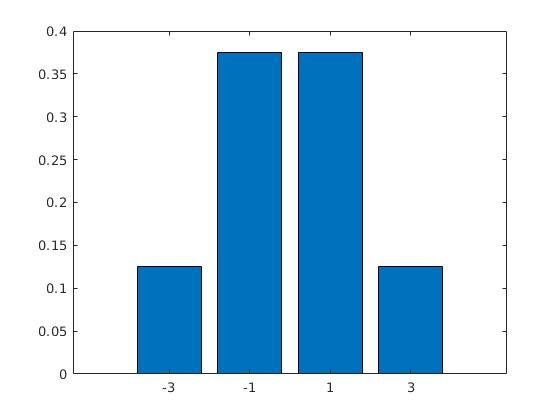
\includegraphics[width=\linewidth]{Q2_D_PMF.jpg}
        \caption{Q2 d) PMF}
    \end{figure}


    \begin{figure}[ht!]
        \centering
        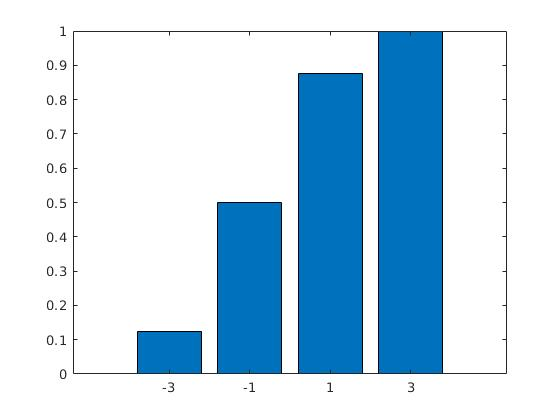
\includegraphics[width=\linewidth]{Q2_D_CDF.jpg}
        \caption{Q2 d) CDF}
    \end{figure}

    \begin{figure}[ht!]
        \centering
        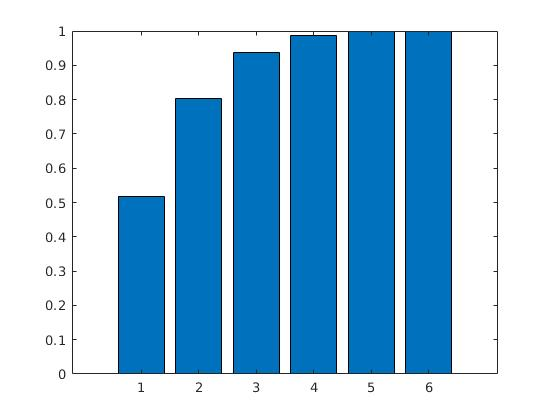
\includegraphics[width=\linewidth]{Q3_c_CDF.jpg}
        \caption{Q3 c) CDF}
    \end{figure}

		
\end{document}




